%!TEX root = Thesis.tex

\chapter{Coordination Complexes with Rhodium and Iridium}
\chaptermark{Rhodium and Iridium}
\label{ch:rhodium}

Rhodium is a very rare element forming only 0.001 ppm of the earth's crust.\cite{Enghag2004Rhabundance}  The majority of the extracted rhodium (81\%) is used in catalytic converters to reduce harmful nitrogen oxides to nitrogen and oxygen.  Another important use of rhodium is in thermocouples where a rhodium-platinum alloyed wire is used, together with a pure platinum wire for use in high-temperature furnaces.\cite{Enghag2004Rh}  Rhodium coordination complexes form active catalysts, most commonly for hydroformylation and hydrogenation.  Wilkinson's catalyst, \ce{[RhCl(PPh3)3]}, is one of the most widely known rhodium catalysts, used mainly for the hydrogenation of alkenes but also for hydroboration of alkenes and selective hydrogenation of $\alpha$-$\beta$-unsaturated carbonyl compounds.  

The 2001 Nobel Prize in Chemistry was awarded to Knowles,\cite{Knowles2002} Noyori\cite{Noyori2002} and Sharpless\cite{Sharpless2002} for their work in asymmetric catalysis, including several examples of rhodium catalysts.  A derivative of Wilkinson's catalyst where triphenylphosphine was replaced by the chiral phosphine (-)-\ce{PMePh^iPr} was reported by Knowles and Sabacky in 1968\cite{Knowles1968}.  This chiral version of Wilkinson's catalyst was the first asymmetric hydrogenation catalyst yielding an enantiomeric excess of 15\% when hydrogenating $\alpha$-$\beta$-unsaturated carbonyls (Scheme \ref{Knowlesscheme}).  This was improved upon by the development of the CAMP ligand (Figure \ref{chiralrhodiumligands}) which gives an enantiomeric excess of 80\% in the hydrogenation of dehydroamino acids, a key step in the commercial production of \iupac{\L-DOPA}  a drug used in the treatment of Parkinson's disease.\cite{Noyori2007}  Rhodium complexes containing chiral diphosphines also form active catalysts, for example a \iupac{[\cip{S}-BINAP}-Rh(COD)] (Figure \ref{chiralrhodiumligands}) catalyst is active for the asymmetric isomerisation of allylic amines a key step in the industrial synthesis of ($-$)-menthol generating over 1000 tons per year.\cite{Noyori2002}

\begin{scheme}[h]
\begin{center}
\vspace{0.5cm}
\includegraphics{../Schemes/Knowlesscheme.eps}
\caption[Asymmetric catalytic hydrogenation developed by Knowles]{Asymmetric catalytic hydrogenation developed by Knowles\cite{Knowles2002}}
\vspace{0.2cm} 
\label{Knowlesscheme}
\end{center}
\end{scheme}
\vspace{0.2cm}

\begin{figure}[h]
\begin{center}
\vspace{0.5cm}
	\begin{subfigure}{0.2\textwidth}
		\includegraphics{../Structures/CAMP.eps}
	\end{subfigure}
	~~~~~~~~~~~~~~~~~~
	\begin{subfigure}{0.2\textwidth}
		\includegraphics{../Structures/BINAP.eps}
	\end{subfigure}
\caption[Chiral phosphine ligands used in asymmetric catalysis]{Chiral phosphine ligands used in asymmetric catalysis.  Left: CAMP, Right: \iupac{\cip{S}-BINAP}}
\vspace{0.2cm}
\label{chiralrhodiumligands}
\end{center}
\end{figure}
\vspace{0.2cm}

%The xantphos class of ligands have long been studied for their role as ancillary ligands in  rhodium catalysed hydroformylation.  

\fixme{include figures of all of the discussed catalysts or ligands}

Xantphos ligands have the ability to coordinate to a metal centre in a number of different modes.  The most common is the diphosphine \dento{2}-\emph{PP\textprime} mode.  Tridentate complexes are also relatively common especially in octahedral complexes typically meridional \POP{} coordination is observed, though facial complexes have also been reported.\cite{Dallanegra2012, Pawley2012}

The xantphos class of ligands were first studied for their potential use as ancillary ligands in rhodium catalysed hydroformylation\cite{Kranenburg1995}.  It was found increasing the bite-angle from 108.7\degrees for sixantphos to 109.4 \degrees for thixantphos and 111.7 \degrees for xantphos resulted in an increase in the selectivity for the linear aldehyde (linear/branched = 35.0, 47.6 and 57.1 respectively).  A more recent paper with \iPrxantphos{} found a dramatic difference between the reactivity of the diphosphine towards rhodium and iridium.  Studying the coordination behaviour of the \tBuxantphos{} ligands with rhodium and iridium thus made logical sense.\fixme{scientific language!}

\section{Synthesis of [Rh(\tBuxantphosk)Cl] complexes}
\label{section:rhodiumchloride}

Rhodium alkene dimers are commonly used starting materials for the formation of rhodium phosphine complexes.  These dimers can react in a number of different ways depending on the phosphine (Figure \ref{RhCOEClcomplexes}.  When two equivalents of a monophosphine react with \ce{[Rh(COE)2Cl]2} the phosphine displaces one cyclooctene molecule from each rhodium forming a symmetric dimer.\cite{Canepa2003}  These complexes are typically unstable.  Further addition of phosphine displace the remaining two cyclooctene molecules while retaining the chloride bridged rhodium core.\cite{Bleeke1986}  Analogous complexes form when the reaction is carried out with diphosphines.\cite{Fryzuk1989}  In some cases bidentate ligands can cleave the dimer resulting in a \ce{[Rh(LL)(COE)Cl]} complex.\cite{Hashimoto2010}  Tridentate ligands are able to cleave the dimer and result in the mononuclear complexes \ce{[Rh(LLL)Cl]}\cite{Khan1988, Hermann2002}.  In the case of negatively charged tridentate ligands the complex forms a trigonal bipyramidal hydride chloride structure (where the hydride forms from the central ligating atom).\cite{Boom1998, Winter2003, Salem2008}  Alternatively the ligand can be reacted first with a strong base or a silver salt can be added to remove the chloride and break the dimer.  In this case the remaining coordination site is occupied by the anion from the silver salt of by a cyclooctene molecule if a non-coordinating counterion is used.\cite{Fryzuk1986, Hanson2008}

\begin{figure}[h!]
\begin{center}
\vspace{0.5cm}
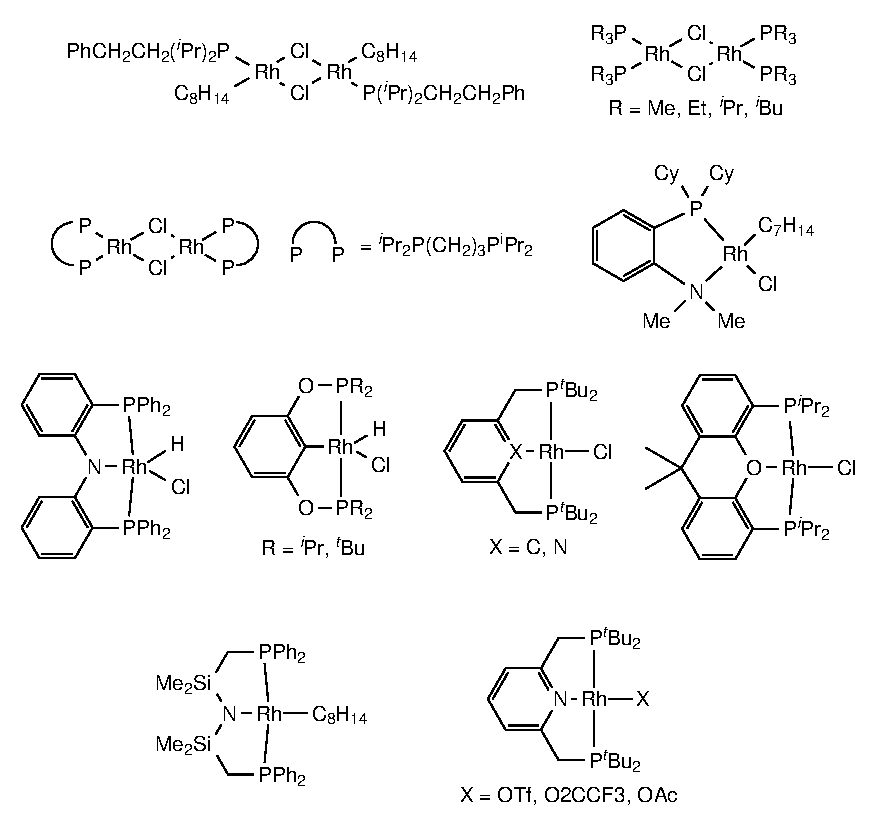
\includegraphics{../Figures/RhCOEClcomplexes.eps}
\caption[Complexes formed by reaction of \ce{[Rh(COE)2Cl]2} and phosphine ligands]{Complexes formed by reaction of \ce{[Rh(COE)2Cl]2} and phosphine ligands.  First row: monophosphines in 2:1 and 4:1 ligand:\ce{[Rh(COE)2Cl]2}, second row: bidentate ligands, third row: tridentate ligands in the absence of other reagents, fourth row: tridentate ligands using lithiated ligand (left) or a silver salt (right).}
\vspace{0.2cm}
\label{RhCOEClcomplexes}
\end{center}
\end{figure}
\vspace{0.2cm}

Reaction between \ce{[Rh(COE)2Cl]2} and the three \tBuxantphos{} ligands was carried out on an NMR scale in \ce{C6D6}.  No reaction occurred at room temperature overnight except in the case of \tBuxantphos{} which displays a small amount of conversion evident from the NMR spectra.  Upon heating to 60 \degC{} the reaction proceeds, going to complete after 24 hours.  For all three \tBuxantphos{} ligands the product is the expected [Rh(\tBuxantphosk)Cl] mononuclear complex (Scheme \ref{RhodiumI}).  This complex is directly analogous to the \iPrxantphos{} complex reported in 2013\cite{Esteruelas2013}.  As seen previously the \tBuxantphos{} ligands have a number of different coordination modes.  In this case a meridional \POP{} pincer coordination is observed.  It is likely the reaction proceeds by substitution of one cyclooctene ligand with one of the phosphorus atoms, followed by a second to form a chloride bridged dimer.  However, as the \tBuxantphos{} have such large bite-angles and the potential coordinating ether bridge this can readily split the dimer resulting in the desired product.  None of these intermediates were observable indicating low activation barriers once the first substitution had occurred.  

\begin{scheme}[htb]
\begin{center}
\vspace{0.5cm}
\includegraphics{../Schemes/RhodiumI.eps}
\caption[Reaction of \ce{[Rh(COE)2Cl]2} and \tBuxantphos{} ligands]{Reaction of \ce{[Rh(COE)2Cl]2} and \tBuxantphos{} ligands.  \tBuxantphos: R = H, X = \ce{CMe2}. \tButhixantphos: R = Me, X = S. \tBusixantphos: R = H, X = \ce{SiMe2}}
\vspace{0.2cm} 
\label{RhodiumI}
\end{center}
\end{scheme}
\vspace{0.2cm}

The NMR spectra for the three complexes is consistent with the proposed structures (spectra for [Rh(\tBuxantphos)Cl] shown in Figure \ref{RhClnmr}) .  In the phosphorus NMR spectra the complexes all display doublets due to rhodium coupling shifted downfield from the free ligand by 35.8-37.5 ppm to 44.2-47.7 ppm with coupling of 140-142.3 Hz (Table \ref{table:rhodiumchloride}).  This coupling is consistent with a rhodium(I) complex and is very close to the coupling for [Rh(\iPrxantphosk)Cl] complex (142.4)\cite{Esteruelas2013}  The \proton{} and \carbon{} NMR spectra support the proposed structure as the \tBu{} proton and carbons all appear as virtual triplets indicating strongly coupled phosphorus atoms which typically occurs in a \trans{} coordination geometry.  In the \carbon{} NMR the O-ipso carbon has shifted downfield relative to the free ligand and similar complexes where the oxygen is known to be non-coordinating [Ag\tBuxantphos)Cl].  This downfield shift is consistent with a coordinated oxygen.  As the oxygen donated electron density to the metal this will inductively decrease electron density on the O-ipso carbon resulting in decreased shielding and thus a downfield shift.  The coupling on the O-ipso carbon decreases from the free ligand to a \dento{2}-\emph{PP\textprime} complex, but increases in the [Rh(\tBuxantphosk)Cl] complexes.  \fixme{why}

\begin{figure}[htbp]
\begin{center}
\vspace{0.5cm}
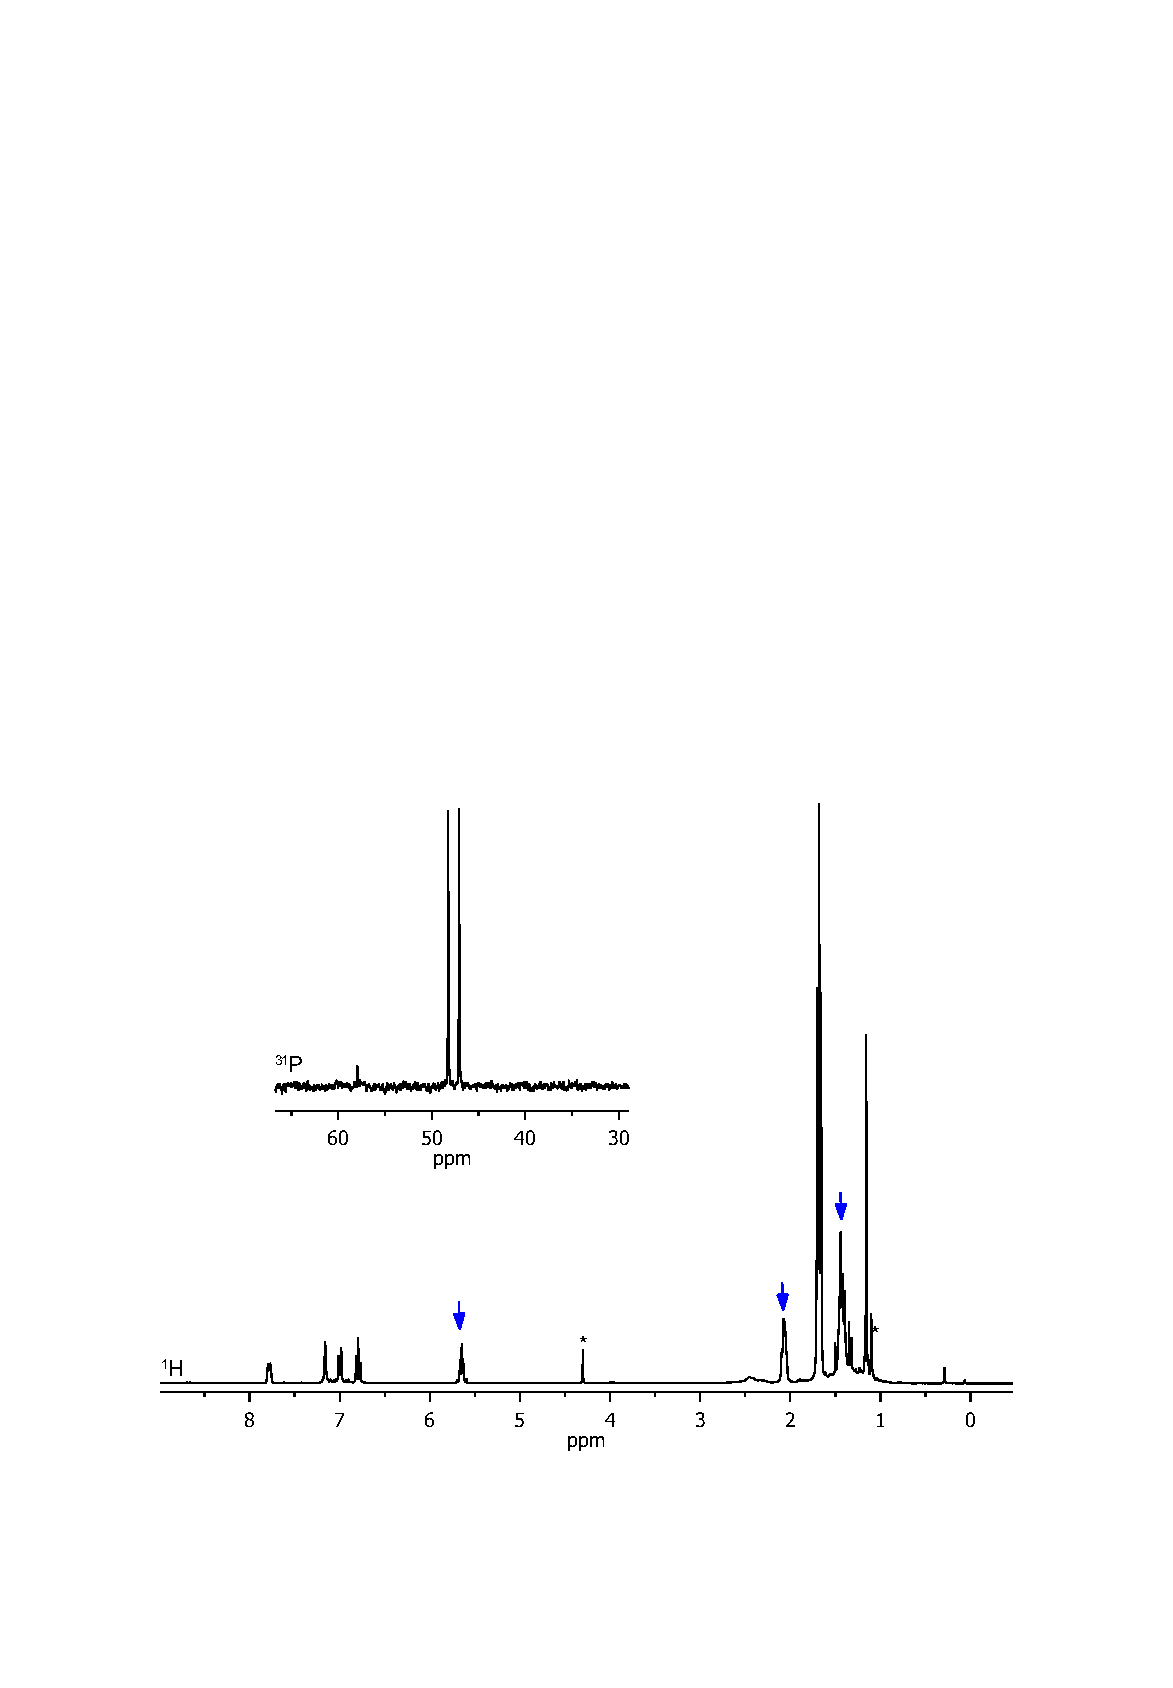
\includegraphics[trim = 2.5cm 4.0cm 2.5cm 15cm, clip]{../NMR/7004B.eps}
\caption[\phosphorus{} and \proton{} NMR spectra for [Rh(\tBuxantphos)Cl{]}]{\phosphorus{} and \proton{} NMR spectra for [Rh(\tBuxantphos)Cl]}
\vspace{0.2cm}
\label{RhClnmr}
\end{center}
\end{figure}
\vspace{0.2cm}

\begin{table}[htbp]
\caption[Selected NMR data of [Rh(\tBuxantphos)Cl{]} complexes]{Selected NMR data of [Rh(\tBuxantphos)Cl] complexes}
\vspace{1em}
\label{table:rhodiumchloride}
\small
\begin{center}
\begin{tabular}{ c c c c c c}
	\toprule{}
	\bfseries{Compound}&\bfseries{$\delta$\phosphorus{}$/$ppm}&\bfseries{$\Delta\delta$}&\bfseries{\JRhP{}$/$Hz}&\bfseries{\proton{} \emph{$^t$}Bu $/$ppm}&\bfseries{\proton{} \emph{$^t$}Bu \J $/$Hz}\\
	\midrule{}
	SitBu	&	44.2	&	35.8	&	140.0	& 1.69	& 13.5\\
	StBu		& 	46.5	&	37.0	&	141.5	& 1.67	& 13.7\\
	CtBu		&	47.7	&	37.5	&	142.3	& 1.68	& 13.4\\
	\bottomrule{}
\end{tabular}
\end{center}
\end{table}

\begin{table}[htbp]
\caption[Chemical shift and coupling of the \emph{O}-ipso carbon when in the free ligand, [Ag(\tBuxantphos)Cl{]} and [Rh(\tBuxantphos)Cl{]} complexes]{Chemical shift and coupling of the \emph{O}-ipso carbon when in the free ligand, [Ag(\tBuxantphos)Cl] and [Rh(\tBuxantphos)Cl] complexes.}
\vspace{1em}
\label{table:oxygenbindingrh}
\small
\begin{center}
\begin{tabular}{ c c c c c c c c c}
	\toprule{}
	~&\multicolumn{2}{c}{\bfseries{Free ligand}} &\multicolumn{3}{c}{\bfseries{[Ag(\tBuxantphos)Cl]}}&\multicolumn{3}{c}{\bfseries{[Rh(\tBuxantphos)Cl]}}\\  
	\bfseries{Ligand}&\bfseries{$\delta$\carbon{}$/$ppm}&\bfseries{\J{} Hz}&\bfseries{$\delta$\carbon{}$/$ppm}&\bfseries{$\Delta\delta$}&\bfseries{\J{} Hz}&\bfseries{$\delta$\carbon{}$/$ppm}&\bfseries{$\Delta\delta$}&\bfseries{\J{} Hz}\\
	\midrule{}
	\tBusixantphos	&	164.3	& 11.3	&	163.9	& -0.4	& 5.2		& 169.5	& 5.2 	& 14.4 \\
	\tButhixantphos	&	155.3	& 13.0	&	155.5	& 0.2 	& 6.6 	& 157.4	& 2.1 	&16.8 \\
	\tBuxantphos	&	155.8	& 12.0	&	156.5	& 0.7		& 6.5		& 158.9	& 3.1		& 16.3 \\
	\bottomrule{}
\end{tabular}
\end{center}
\end{table}

%A reaction occurs rapidly with all three diphosphine to form complexes \fixme{compound reference} (Scheme \ref{RhodiumI}).  These complexes have \JRhP{} coupling constants of around 142 Hz, consistent with rhodium(I).  The complexes are direct analogues of those reported for \iPrxantphos{} which has a \JRhP{} coupling constant of 142.4 Hz.\cite{Esteruelas2013}  The \tBuxantphos ligands are coordinated in a tridentate manner with the oxygen binding.  In the \carbon{} NMR spectrum this can be seen as the O-ipso carbon carbon has shifted to downfield.  For example in \tBuxantphos{} this carbon resonants at 155.8 ppm, in the complex \ce{[(tBu-xantphos)AgCl]} the carbon shifted to 156.5 although the oxygen was not binding.  In the tridentate rhodium complex this carbon has moved downfield again to 158.9 ppm.  This shift in the resonant frequency of this carbon is a result of the oxygen donating electron density to the rhodium, which in turn makes the oxygen withdraw electron density from the ipso carbons.  

\section{Reaction with Hydrogen}
\label{section:rhodiumhydride}

Rhodium complexes are well-known as homogeneous hydrogenation and hydroformylation catalysts.  Both of these processes involve the activation of molecular hydrogen at the rhodium centre.  The catalytic cycle for hydrogenation using monophosphine ligands (Scheme \ref{Hydrogenationcycle}) involves the addition of molecular hydrogen to \ce{[Rh(PR3)2Cl]} generating a rhodium dihydride, which then coordinates an alkene and hydride-migration and \chembeta-hydride elimination to generate the starting rhodium complex and the alkane.  Whilst in hydroformylation (Scheme \ref{Hydroformylationcycle}) the alkene in coordinated to an existing rhodium hydride complex.  Hydride migration occurs followed by carbon monoxide coordination and migratory insertion into the rhodium alkyl bond.  This is followed by the oxidative addition of dihydrogen, generating a rhodium(III) dihydride complex.  The cycle concludes by \chembeta-hydride elimination generating the aldehyde and the starting rhodium(I) complex.  Hydroformylation was the first catalytic process that the influence of the bite-angle of various xantphos complexes was studied\cite{Kranenburg1995} and has since been studied extensively.\fixme{citations}  Given the importance of the oxidative addition of molecular hydrogen for both of hydrogenation and hydroformylation we investigated the reactivity of the [Rh(\tBuxantphosk)Cl] complexes with dihydrogen.  

\begin{scheme}[htbp]
\begin{center}
\vspace{0.5cm}
\includegraphics{../Schemes/Homogeneoushydrogenation.eps}
\caption[Catalytic cycle for homogeneous hydrogenation]{Catalytic cycle for homogeneous hydrogenation using a rhodium chloride complex with monophosphine ligands}
\vspace{0.2cm}
\label{Hydrogenationcycle}
\end{center}
\end{scheme}

\begin{scheme}[htbp]
\begin{center}
\vspace{0.5cm}
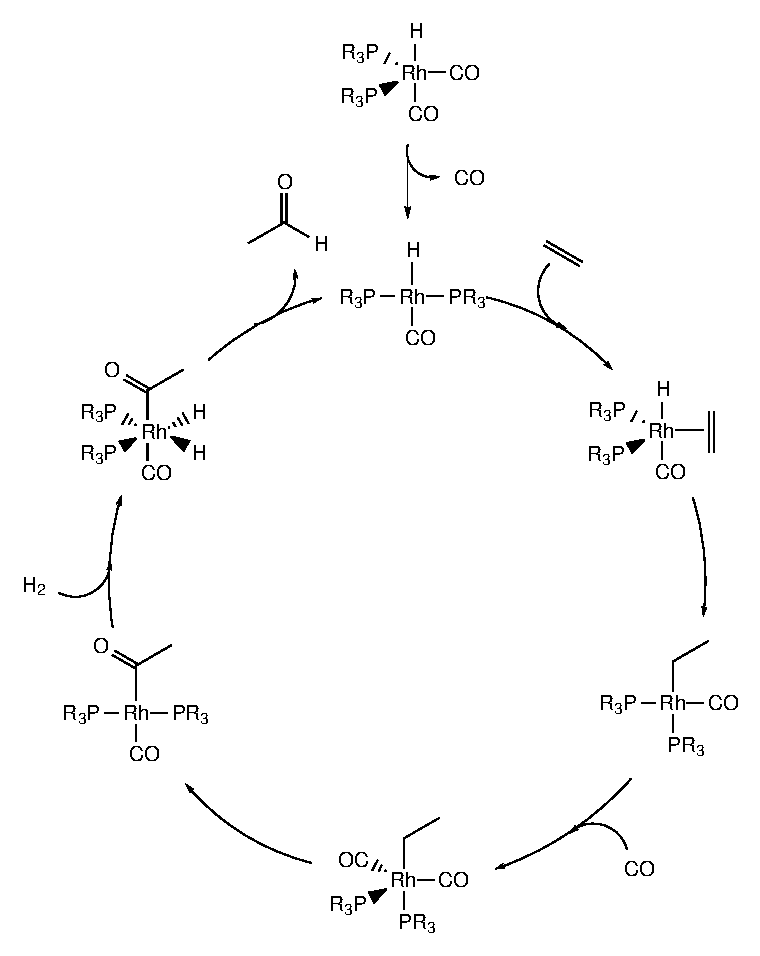
\includegraphics{../Schemes/Hydroformylationcycle.eps}
\caption[Catalytic cycle for homogeneous hydroformylation using diphosphine ligands]{Generic catalytic cycle for homogeneous hydroformylation using diphosphine ligands}
\vspace{0.2cm}
\label{Hydroformylationcycle}
\end{center}
\end{scheme}

The complexes [Rh(\tBuxantphosk)Cl] are reactive towards hydrogen, readily splitting the hydrogen to form octahedral rhodium(III) dihydride complexes (Scheme \ref{Rhodiumhydride}).  The hydrogen is split to form to different hydride environments in the product with a \cis{} arrangement.  The \tBuxantphos{} ligands retain their meridional coordination however, the two faces of the ligand are now different results in two different environments for the methyls in both \tBusixantphos{} and \tBuxantphos{}, and the \tBu{} groups.  

\begin{scheme}[htbp]
\begin{center}
\vspace{0.5cm}
\includegraphics{../Schemes/Rhodiumhydride.eps}
\caption[Reaction of \ce{[Rh(tBu-xantphos)Cl]} with hydrogen]{Reaction of \ce{Rh(tBu-xantphos)Cl]} with hydrogen.  tBu-xantphos: R = H, X = \ce{CMe2}. tBu-thixantphos: R = Me, X = S. tBu-sixantphos: R = H, X = \ce{SiMe2}}
\vspace{0.2cm} 
\label{Rhodiumhydride}
\end{center}
\end{scheme}
\vspace{0.2cm}

Two hydride resonances are evident in the \proton{} NMR spectra occurring upfield as well defined doublets of triplets of doublets coupling to the rhodium, two phosphorus atoms and the each other (Figure \ref{rhodiumhydridenmr}, Table \ref{table:dihydrides}).  The hydride \emph{trans} to the chloride ligand (-16.92 to -17.04 ppm) shows very little change in either the chemical shift or coupling constants for the three complexes.  The hydride \trans{} to the \tBuxantphos{} oxygen (-20.51 to -21.12 ppm) shows more variance in the chemical shift and coupling.  The value \JRhH{} decreases with increasing natural bite-angle.  As the bite-angle for the \tBuxantphos{} ligand increases, the ligand will require less energy to adopt a pincer coordination mode.  This results in the larger bite-angle ligands adopting a mode closer to the ideal T-shaped pincer coordination causing a smaller Rh-O bond length.  This stronger bond in the \trans{} position results in a decreased coupling constant for the hydride ligand.  

\begin{figure}[htbp]
\begin{center}
\vspace{0.5cm}
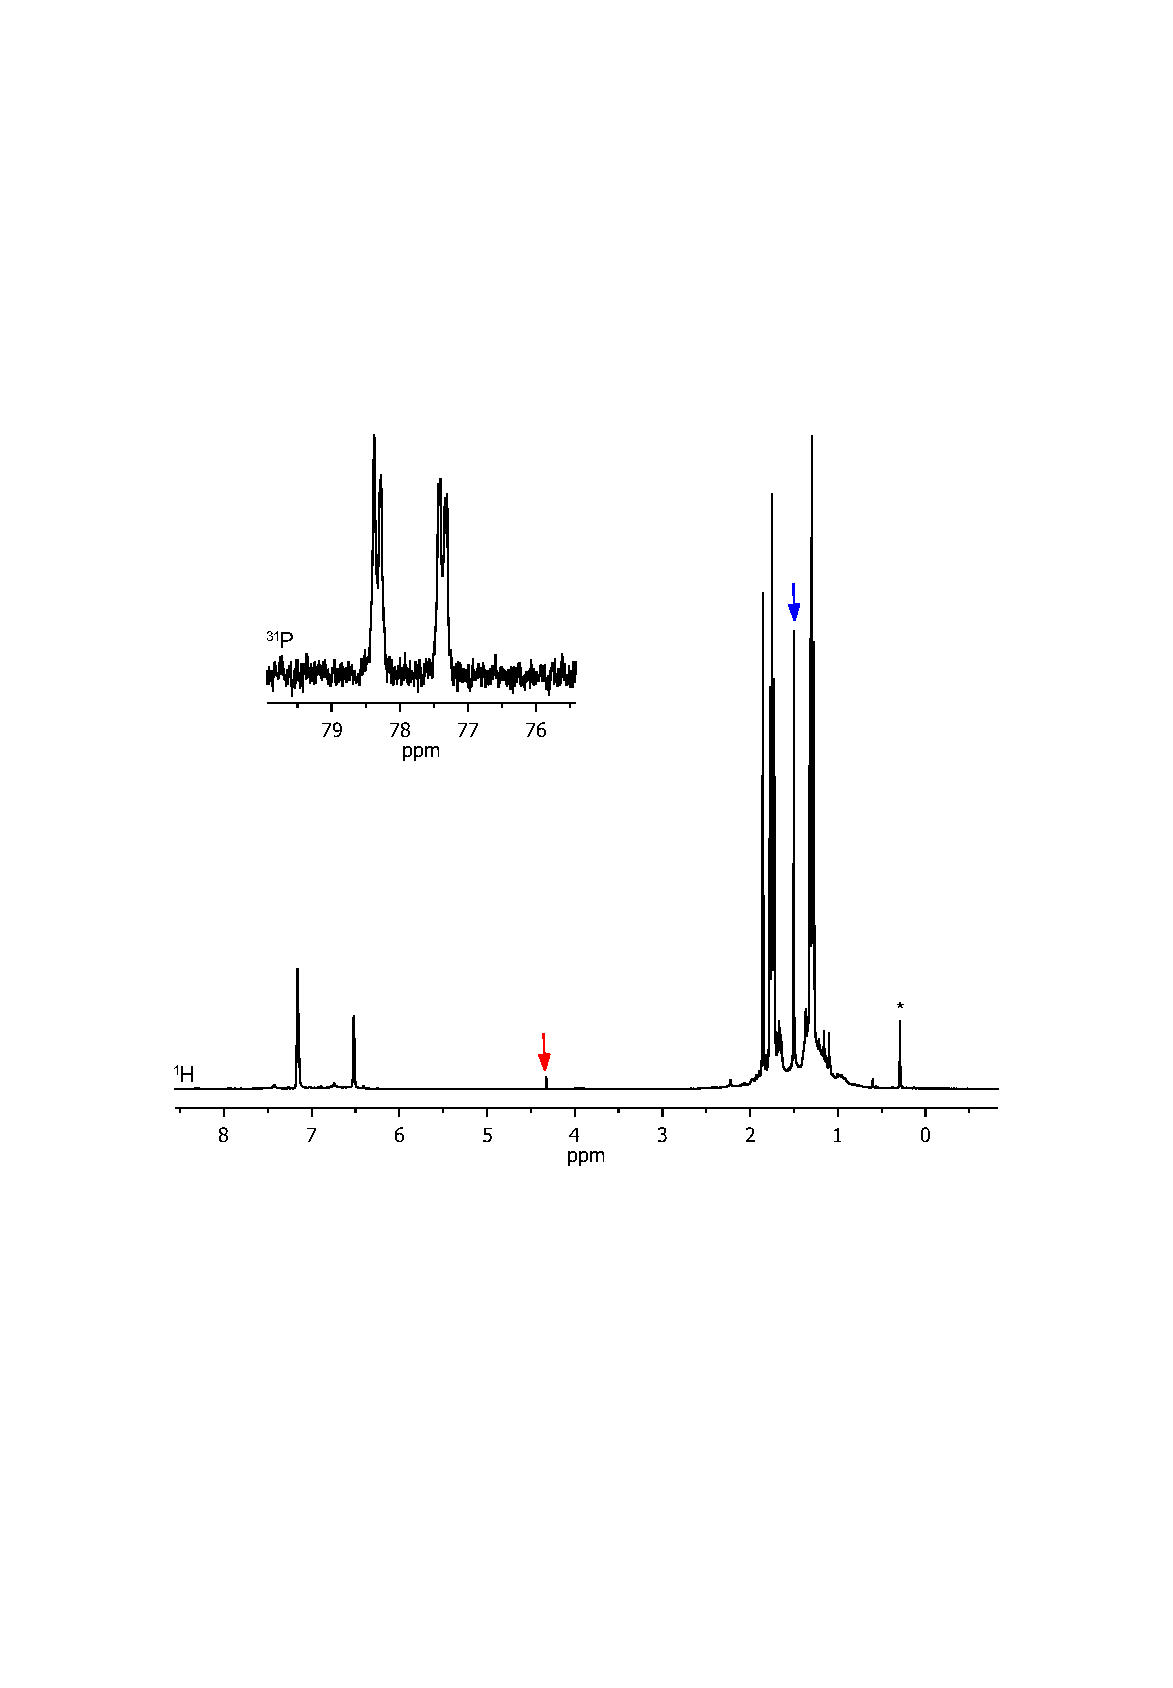
\includegraphics[trim = 2.5cm 8.5cm 2.5cm 7.0cm, clip]{../NMR/7006E.eps}
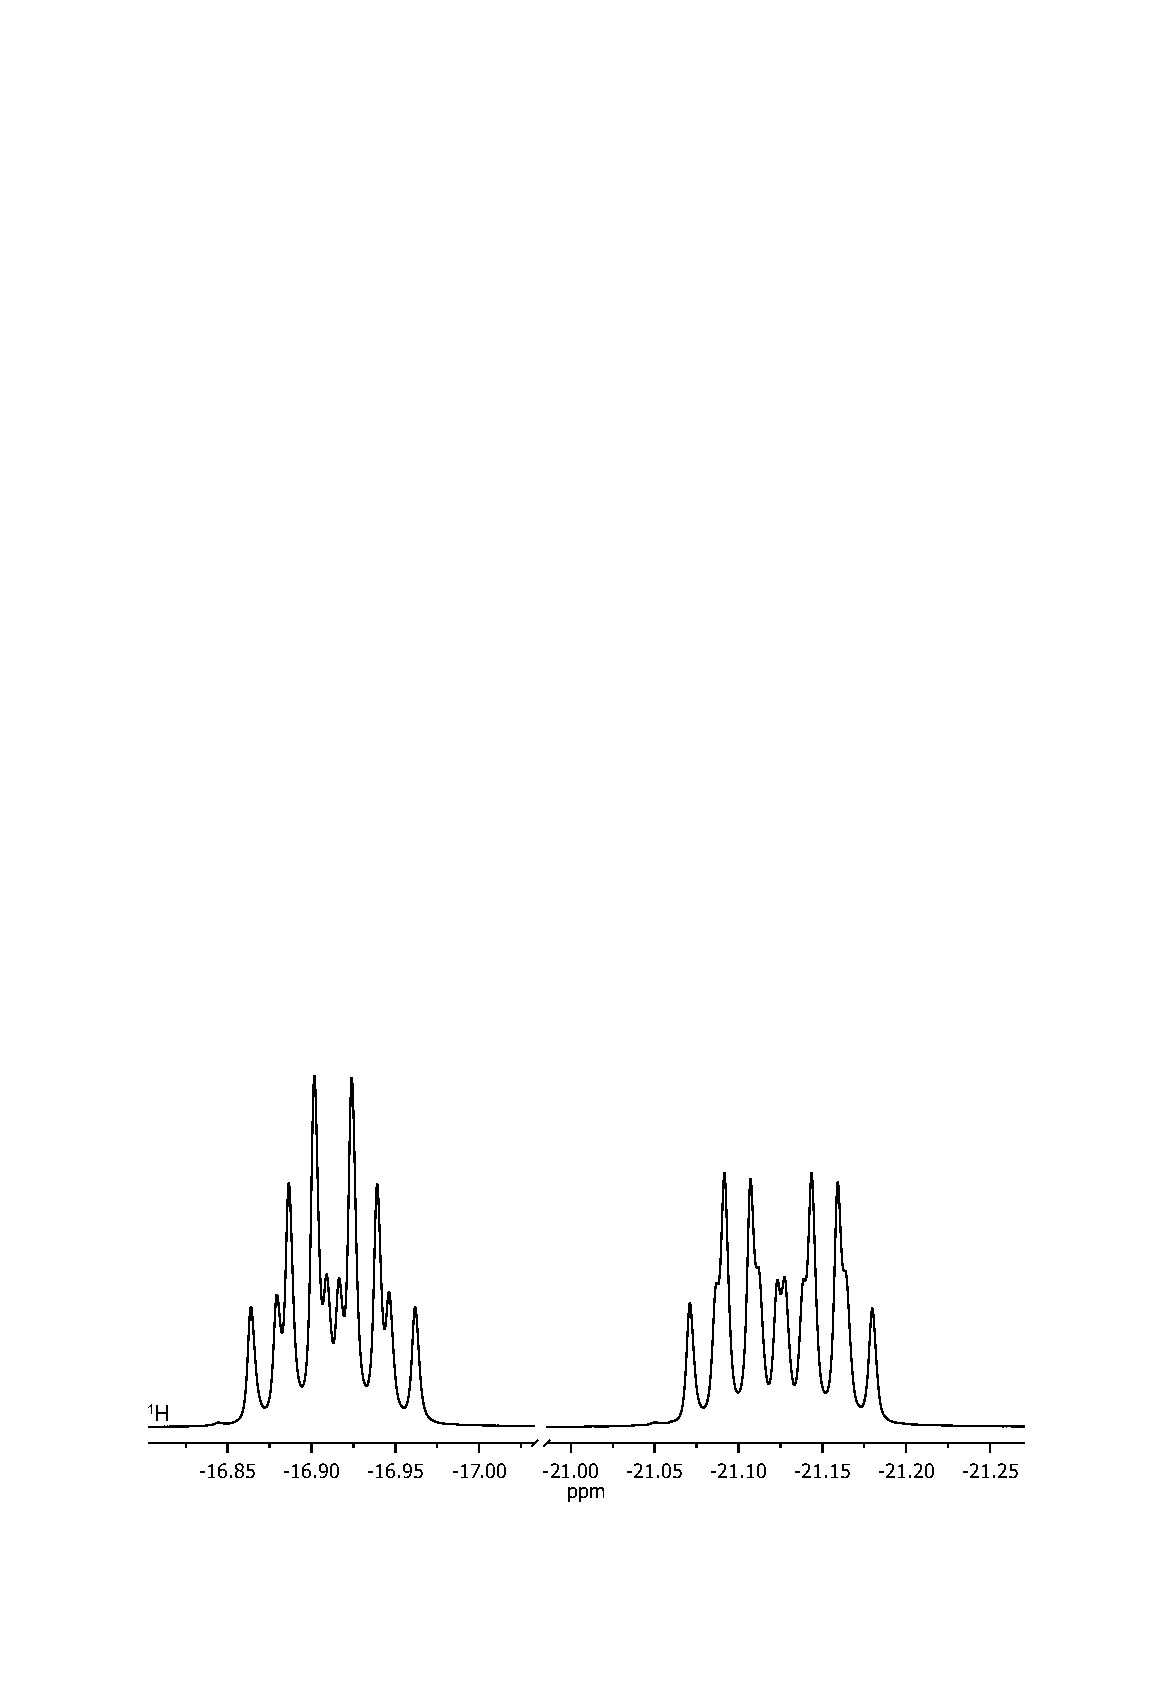
\includegraphics[trim = 2.0cm 2.5cm 2.0cm 17cm, clip]{../NMR/7007.eps}
\caption[NMR spectra for \ce{[Rh(\tButhixantphos)Cl(H)2]}]{NMR spectra for \texorpdfstring{[Rh(\tButhixantphos)\ce{Cl(H)2]}} R.  Impurities are indicated by *, \ce{CH2Cl2} is indicated by a red arrow and cyclooctane by a blue arrow.\fixme{the hydrides are for Si while the rest is S}}
\vspace{0.2cm}
\label{rhodiumhydridenmr}
\end{center}
\end{figure}
\vspace{0.2cm}

\begin{sidewaystable}
\caption[Hydride \proton{} NMR data for \ce{[Rh(\POP)Cl(H)2]}]{Hydride \proton{} NMR data for \texorpdfstring{\ce{[Rh(\POP)Cl(H)2]}}R}
\vspace{1em}
\label{table:dihydrides}
\small
\begin{center}
\begin{tabular}{c c c c c c c c c}
\toprule{}
	~~ & \multicolumn{4}{c}{\bfseries{\ce{H-} \trans-\ce{Cl-}}} & \multicolumn{4}{c}{\bfseries{\ce{H-} \trans-O}}\\
	\bfseries{Diphosphine}&\bfseries{$\delta/$ppm}&\bfseries{\JRhH$/$Hz}&\bfseries{\JPH$/$Hz}&\bfseries{\JHH$/$Hz}&\bfseries{$\delta/$ppm}&\bfseries{\JRhH$/$Hz}&\bfseries{\JPH$/$Hz}&\bfseries{\JHH$/$Hz}\\
	\midrule{}
	\tBuSixantphos & -16.92 & 22.7 & 13.5 & 9.4 & -21.12 & 30.9 & 12.1 & 9.2 \\
	\tBuThixantphos & -17.00 & 22.6 & 13.5 & 9.4 & -21.13 & 30.5 & 12.4 & 9.4 \\
	\tBuXantphos & -17.04 & 22.8 & 13.4 & 9.4 & -20.51 & 28.8 & 12.2 & 9.4 \\
	\bottomrule{}
\end{tabular}
\end{center} 
\end{sidewaystable}

The \phosphorus{} NMR spectra (Figure \ref{rhodiumhydridenmr}) for the [Rh(\tBuxantphosk)\ce{(H)2Cl]} complexes each display a single resonance downfield relative to the starting [Rh(\tBuxantphosk)Cl] complexes as a doublet of doublets with some further coupling evident.  Although \phosphorus{} NMR is \proton{} decoupled the decoupler is unable to decouple resonances that are so far outside the typical \proton{} range (-2 to 15 ppm) resulting in the residual coupling.  The value of \JRhP{} has decreased by 23.7-25.3 Hz to 116.1-117.8 Hz consistent with a change in the oxidation state of the rhodium centre from Rh(I) to Rh(III).  Consistent with the proposed geometry, the \proton{} NMR spectra also display two signals for the \tBu{} protons, both appearing as virtual triplets indicating the \trans{} coordination of the phosphorus atoms.  Two signals were also observed in the \proton{} NMR spectra for the bridgehead methyls in [Rh(\tBuxantphosk\ce{)(H)2Cl]} and [Rh(\tBusixantphosk\ce{)(H)2Cl]}, again consistent with the proposed structure.  

The reported [Rh(\tBuxantphosk\ce{)(H)2Cl]} complexes are similar to previously reported dihydride complexes of \iPrxantphos{}\cite{Esteruelas2013, Esteruelas2013b} and \Phxantphos{}\cite{Dallanegra2012, Johnson2013, Pawley2010}.   In these cases the hydride \trans{} to the oxygen atom was located in the \proton{} NMR between -22.19 and -19.00 ppm with a rhodium coupling constant of 27.0 - 33.8 Hz.  The \proton{} NMR signals for the hydride in the newly reported [Rh(\tBuxantphosk\ce{)(H)2Cl]} complexes are encompassed within these ranges (Table \ref{table:dihydrides}).  For the reported \tBuxantphos{} complexes the \phosphorus{} chemical shift is 77.8-79.0 ppm with \JRhP{} = 116.1-117.8 Hz.  In comparison the literature complexes appear at 36.9-45.4 ppm and \JRhP{} = 114-121 for \Phxantphos{} and 64.8-67.2 ppm and 113-114 Hz for \iPrxantphos{}.  The coupling constants are consistent for the complexes, and although the absolute chemical shift varies significantly, the change in chemical shift from the [Rh(I)(POP)Cl] complexes is consistent (28.7-31.1 ppm for \iPrxantphos{} compared to 31.3-34.0 ppm for \tBuxantphos{}, [Rh(\Phxantphos)Cl] has not been reported in the literature).  

In some cases with \Phxantphos{} the complexes were reportedly only stable under a hydrogen atmosphere,\cite{Johnson2013, Dallanegra2012} however, in the case of \tBuxantphos{} the complexes were able to be placed under vacuum overnight with no evidence for loss of hydrogen.  This difference is likely the result of the different electronics between \tBuxantphos{} and \Phxantphos{}.  The electron donating nature of the \tBu{} groups on \tBuxantphos{} enhances electron donation from the rhodium centre into the $\sigma$* orbital of a dihydrogen ligand, thus favouring oxidative addition and the formation of two discrete hydrides.  As the \Phxantphos{} has two electron withdrawing phenyl substituents on each phosphorus atom together with the aromatic backbone of the ligand this will have less back-bonding and thus less of a barrier towards the reformation of a dihydrogen ligand which could dissociate under vacuum.  \fixme{citations for electron donating vs electron withdrawing}

The synthesis of [Rh(\tBuxantphosk)Cl] from \ce{[Rh(COE)2Cl]2} generates free cyclooctene as a by-product.  This reaction mixture was used without further purification to determine the potential for the [Rh(\tBuxantphosk)Cl] complexes to act as hydrogenation catalysts.  Hydrogen gas was bubbled through a mixture of [Rh(\tBuxantphosk)Cl] and cyclooctene for 10 minutes before the reaction was sealed and allowed to proceed at room temperature.  After \fixme{some amount of time} no evidence for cyclooctene was observed by \proton{} NMR spectroscopy in the reaction mixture and a peak for cyclooctane was apparent (Figure \ref{rhodiumhydridenmr}).  While further work to determine the activity of these complexes needs to be performed, this result indicates the potential for the [Rh(\tBuxantphosk)Cl] to act as precatalyts for hydrogenation of alkenes.  

\fixme{get time periods etc.}

%The hydrides appear as two signals in the \proton{} NMR spectrum upfield at -17.12 ppm and -20.54 ppm (dtd, \JRhH = 28.7, \JPH = 12.1, \JHH = 9.1) \fixme{give coupling constants} as doublets of triplets of doublets coupling to the rhodium, two phosphorus' and the other hydride.  \fixme{put in a picture of this because it's kind of awesome}  This downfield shift of the O-ipso carbon is retained at \fixme{value} indicating that the tridentate coordination of the xantphos ligand is retained.  This reaction appears to be reversible an equilibrium such that at 1 atm of hydrogen a ratio of \fixme{value} between the two species is observed.  Over time as the hydrogen dissipates out of the NMR tube the reaction returns to starting material.  In addition this complex does convert to the unknown rhodium(III) species over time.  This is likely due to the hydrogen dissipating resulting in return to the rhodium(I) species which then reacts to the unknown rhodium(III) complex.

\subsection{Protonation of \texorpdfstring{[Rh(\tButhixantphos)\ce{Cl(H)2]}} R Complexes}

In order for molecular hydrogen to oxidatively add to the rhodium centre it must first coordination as an \hapto{2}-dihydrogen ligand.  Since their discovery by Kubas in 1984\cite{Kubas1984} several hundred dihydrogen complexes have been reported.\cite{McGrady2003}  However, despite their implication as intermediates in a number of catalytic processes including hydrogenation and hydroformylation rhodium complexes of \hapto{2}-dihydrogen are surprisingly rare.  Dihydrogen coordinates to a metal centre by donation from the H-H $\sigma$-bonding orbital to the metal centre and back-donation from the metal into the H-H $\sigma*$ orbital.  Thus complexes of the late transition metals, especially those with strongly electron donating phosphines such as \tBuxantphos{} result in the oxidative addition of hydrogen rather than coordination as a dihydrogen moiety.  However, dihydrogen complexes can also be synthesised by protonation of preformed metal hydride complexes.  First reported as a synthetic method by Crabtree and coworkers in 1986\cite{Crabtree1986} this method has since been used to create numerous dihydrogen complexes\cite{Janak2004, Oldham1997, Pons2004, Heinekey1993}.

%The rhodium dihydride complexes are stable and do not need to be stored under a hydrogen atmosphere, showing no degradation after storing under argon.  These complexes are not air-stable however as will be discussed in Section \ref{section:rhodium oxygen}. 

As previously discussed the addition of molecular hydrogen to the [Rh(\tBuxantphosk)Cl] complexes resulted in cleavage of the H-H bond and formation of the dihydride complexes [Rh(\tBuxantphosk)\ce{(H)2Cl]}.  These dihydride complexes were treated with one equivalent of the strong acid, \ce{CH2(SO2CF3)2}, or \ce{HBF4.OEt2}.  With either acid and all three \tBuxantphos{} ligands the \phosphorus{} NMR spectra showed negligible change (Table \ref{table:dihydrogen}).  In the \proton{} NMR spectrum the aromatic signals are unchanged.  However, the \tBu{} resonances had changed from two virtual triplets to a broad singlet.  A similar effect was observed for the methyl signals in \tBuxantphos{} and \tBusixantphos{}, but not for \tButhixantphos{} as its methyl groups were already equivalent.  The resonances attributed to the hydride signals in [Rh(\tBuxantphosk)\ce{(H)2Cl]} were well-resolved doublets of triplets of doublets.  Upon protonation these were replaced by two broad resonances with essentially no change in chemical shift.  When protonation was carried out with \ce{CH2(SO2CF3)2} the \fluorine{} NMR showed a singlet peak at between -76.2 and -76.4 ppm indicative of the non-coordinated \ce{CH(SO2CF3)2-} anion.

The NMR data from the protonation of [Rh(\tBuxantphosk)\ce{(H)2Cl}] with \ce{CH2(SO2CF3)2} shows very little change except for some broadening of parts of the spectrum.  From this we propose that the an equilibrium state is achieved between a number of different species however, this equilibrium heavily favours the initial dihydride complex.  Rhodium dihydrogen complexes with additional hydride ligands frequently display exchange of the dihydrogen and hydride sites in the complex.\fixme{get a reference}  In this case we may also see reversible loss of HCl which would result in the two faces of the complex being equivalent.  This HCl could then re-protonate the complex resulting in the initial dihydrogen hydride chloride complex.  \fixme{draw a scheme}

When \ce{HBF4.OEt2} was used instead of \ce{CH2(SO2CF3)2} a peak for the free \ce{BF4-} counterion was not observed (expected =151 ppm\cite{Feller2007})  Instead the \fluorine{} NMR spectrum showed a number of peaks between -142 and -156 ppm, some of these peaks were of similar intensities indicating the possibility of coupling to a rhodium centre.  In this case the \proton{} NMR is very similar to that for the reaction with \ce{CH2(SO2CF3)2} indicating that an equilibrium has likely been established.  In this case however, once the chloride has dissociated a \ce{BF4-} ligand may coordinate in its place resulting in the mixture of species observed in the \fluorine{} NMR spectrum.   However, rhodium complexes with monodentate \ce{BF4-} ligands coordinated through one of the fluorine atoms generally come between -164 and -160 ppm in the \fluorine{} NMR spectrum.\cite{Feller2007, Salem2006, Salem2008, Gandelman2003}

%Negligible difference was observed in the \phosphorus{} NMR spectrum and the aromatic resonances of the \proton{} and \carbon{} NMR spectra (Table \ref{table:dihydrogen}).  However, the resonances for the \tBu{} and hydridic protons and carbons are very broad, coalescing to a single broad peak for the \tBu{} protons and two broad peaks for the \tBu{} carbons.  The hydridic protons appear in the same position as the dihydride however the well-resolved doublets-of-triplets-of-doublets have been replaced by two very broad singlets. 

\begin{table}[htbp]
\caption[Selected NMR data of rhodium dihydride and dihydrogen complexes]{Selected NMR data of rhodium dihydride and dihydrogen complexes} 
\vspace{1em}
\label{table:dihydrogen}
\small
\begin{center}
\begin{tabular}{ c c c c c}
	\toprule{}
	~~ & \multicolumn{2}{c}{\bfseries{Dihydride}} & \multicolumn{2}{c}{\bfseries{Protonated}}\\
	\bfseries{Diphosphine}&\bfseries{$\delta$\phosphorus{}$/$ppm}&\bfseries{\JRhP$/$Hz}&\bfseries{$\delta$\phosphorus{}$/$ppm}&\bfseries{\JRhP$/$Hz}\\
	\midrule{}
	SitBu	&	78.2	&	116.1	&	78.1		&	115.6\\
	StBu		& 	77.8	&	117.8	&	77.7		&	115.7\\
	CtBu		&	79.0	&	117.0	&	78.9		&	115.6\\
	\bottomrule{}
\end{tabular}
\end{center}
\end{table}


\section{Rhodium Carbonyl Complexes}

\begin{figure}[htb]
\begin{center}
\vspace{0.5cm}
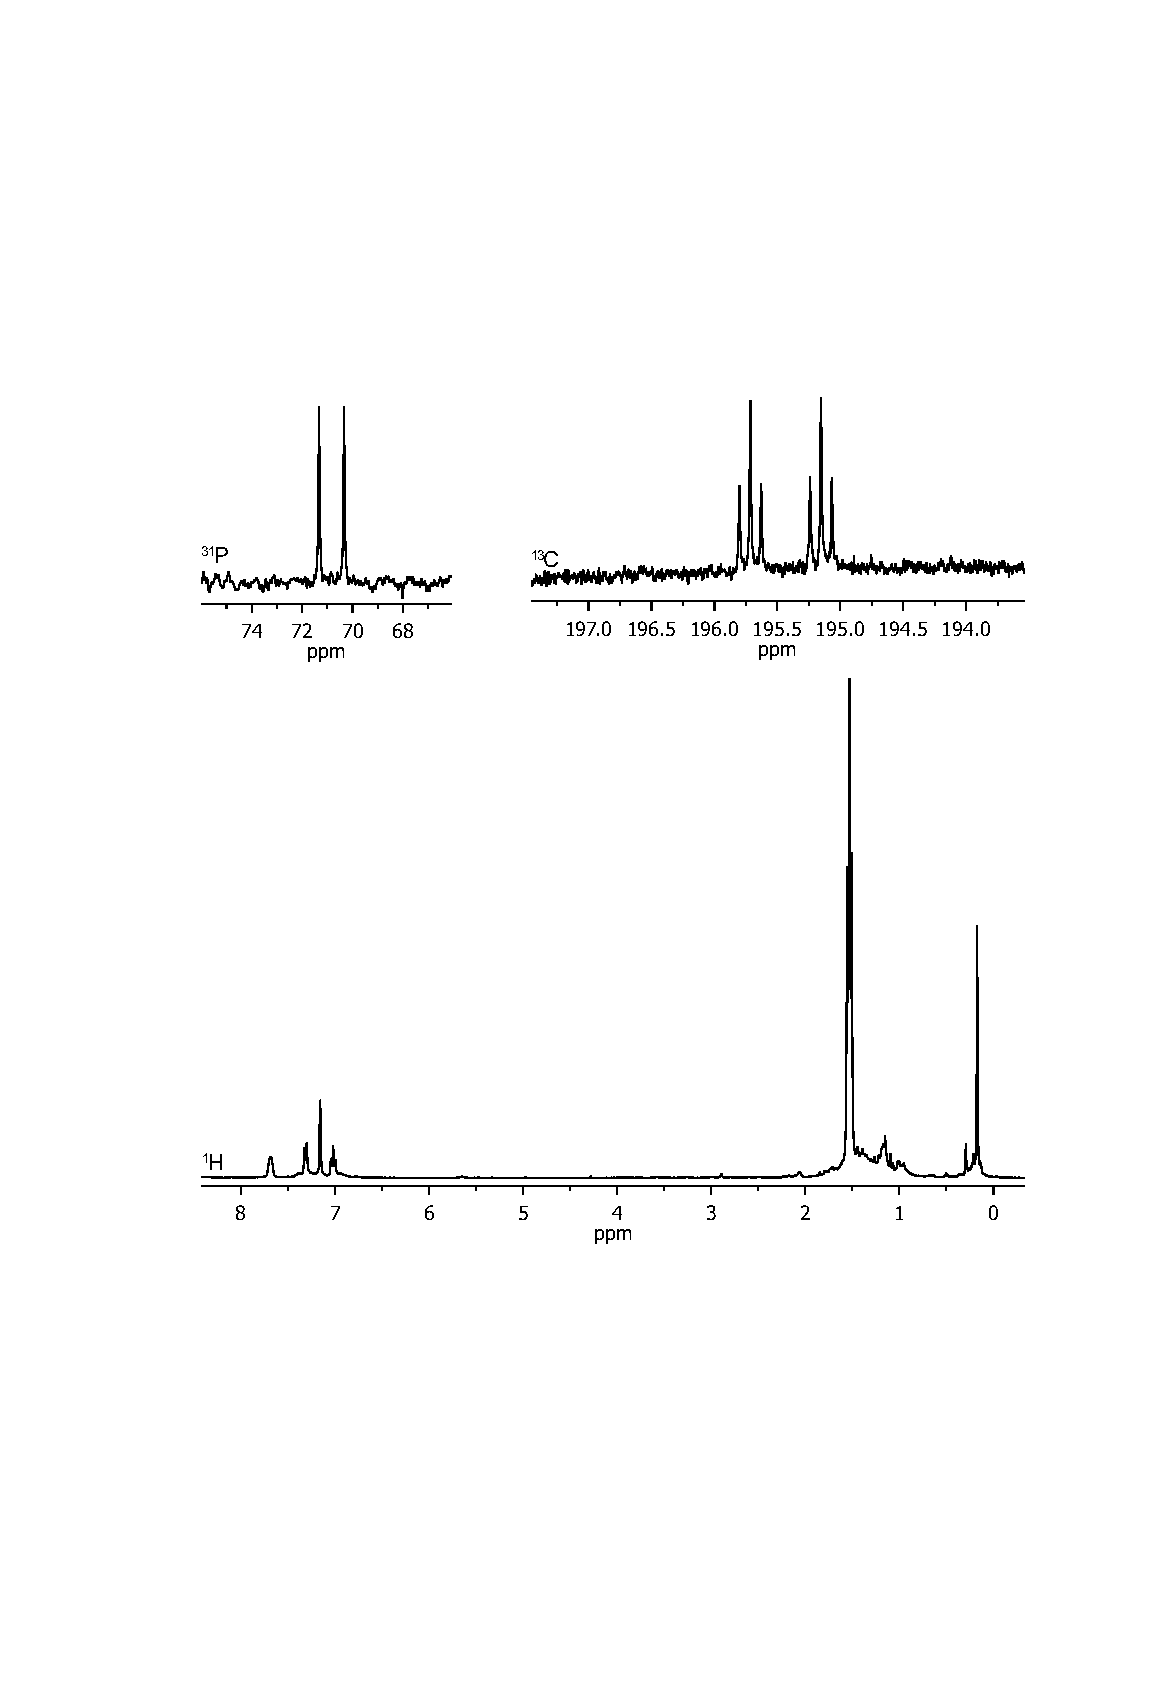
\includegraphics[trim = 2.5cm 7.2cm 2.5cm 5.0cm, clip]{../NMR/7017.eps}
\caption[\phosphorus{} and \proton{} NMR spectra for [Rh(\tBuxantphos)Cl{]}(CO)2]{\phosphorus{} and \proton{} NMR spectra for \ce{[Rh(\tBuxantphos)Cl(CO)2]}}
\vspace{0.2cm}
\label{Rhcarbonylnmr}
\end{center}
\end{figure}
\vspace{0.2cm}

\section{Dioxygen and Oxo Complexes}

Unlike the complexes with iPr-xantphos the complexes \ce{[Rh($\eta^3-$tBu-xantphos)Cl]} were unstable in solution over prolonged periods.  Overnight a new resonance appeared in the \phosphorus NMR spectrum, shifted upfield with a much smaller coupling constant (\JRhP{} = 101.5 Hz).  This decrease in coupling constant is consistent with an increase in the oxidation state to rhodium(III).  However, this occurred in dry, degassed\ce{C6D6} which should not be reactive towards the complex.  No signals other than those expected for the ligand were observed in the \proton, \carbon, or \phosphorus{} NMR spectra.  

Dark red crystals were obtained by slow evaporation of a benzene solution of the unknown rhodium(III) complex.  The crystal structure (Figures \ref{Crystal:rhodium} and \ref{Crystal:rhodiumside}) revealed the presence of a coordinated dioxygen molecule.  The complex crystallised as \ce{[Rh(tBu-xantphos)Cl(}$\eta_2$\ce{-O2})] in the orthorhombic space group \emph{Pbca}.  Selected bond lengths and angles are given in Table \ref{crystal:rhodium:lengths} and crystallographic data is given in Table \ref{crystal:rhodium:data}.  This complex likely formed by slow diffusion of oxygen through the septum sealing the NMR tube.  The crystal structure showed some substitutional disorder with the peroxo ligand substituted for an oxo ligand in approximately 15\% of the sites.  Selected bond lengths and angles for the oxo complex are given in Table \ref{crystal:rhodium:lengths:oxo}.

%\begin{figure}[htp]
%\begin{center}
%\vspace{0.5cm}
%\includegraphics[width=0.6\textwidth]{../Figures/Crystalrhodium.pdf}
%\caption[X-ray crystal structure of \ce{[Rh(tBu-xantphos)Cl(}$\eta^2$\ce{-O2}){]}]{X-ray crystal structure of \ce{[Rh(tBu-xantphos)Cl(}$\eta^2$\ce{-O2})], hydrogen atoms omitted for clarity.}
%\vspace{0.2cm}
%\label{Crystal:rhodium}
%\end{center}
%\end{figure}
%\vspace{0.2cm}

%\begin{figure}[htp]
%\begin{center}
%\vspace{0.5cm}
%\includegraphics[width=0.4\textwidth]{../Figures/Crystalrhodiumside.pdf}
%\caption[X-ray crystal structure of \ce{[Rh(tBu-xantphos)Cl(}$\eta^2$\ce{-O2}){]} - side view]{X-ray crystal structure of \ce{[Rh(tBu-xantphos)Cl(}$\eta^2$\ce{-O2})], hydrogen atoms omitted for clarity - side view}
%\vspace{0.2cm}
%\label{Crystal:rhodiumside}
%\end{center}
%\end{figure}
%\vspace{0.2cm}

\begin{table}[htp]
\caption[Selected bond distances (\AA) and angles (\degrees) of \ce{[Rh(tBu-xantphos)Cl(}$\eta^2$\ce{-O2}){]}]{Selected bond distances (\AA) and angles (\degrees) of \ce{[Rh(tBu-xantphos)Cl(}$\eta^2$\ce{-O2})]}
\vspace{1em}
\label{crystal:rhodium:lengths}
\small
\begin{center}
\begin{tabular}{l l l l}
	\toprule
	\multicolumn{2}{l}{\bfseries{~Bond distances (\si{\angstrom})}} & \multicolumn{2}{c}{\bfseries{Bond angles (\degrees)}} \\
	\midrule		
%	~P1-O2		~~&~~XXXX~~	&~~					&~~XXXX~~	\\
%	~P1-O2		~~&~~XXXX~~	&~~					&~~XXXX~~	\\
%	~P1-O2		~~&~~XXXX~~	&~~					&~~XXXX~~	\\
%	~P1-O2		~~&~~XXXX~~	&~~					&~~XXXX~~	\\
%	~P1-O2		~~&~~XXXX~~	&~~					&~~XXXX~~	\\
%	~P1-O2		~~&~~XXXX~~	&~~					&~~XXXX~~	\\
%	~P1-O2		~~&~~XXXX~~	&~~					&~~XXXX~~	\\
	~O1-Pt		~~&~~3.565~~	&~~Ring 1-Ring 2		&~~XXXX~~		\\
	~O2-Pt		~~&~~3.497~~	&~~Ring 3-Ring 4		&~~XXXX~~		\\
%	~P1-O2		~~&~~XXXX~~	&~~					&~~XXXX~~	\\
%	~P2-O2		~~&~~XXXX~~	&~~					&~~XXXX~~	\\
%	~P3-O1		~~&~~XXXX~~	&~~					&~~XXXX~~	\\
%	~P4-O1		~~&~~XXXX~~	&~~					&~~XXXX~~	\\
	\bottomrule{}
\end{tabular}
\end{center}
\end{table}

\begin{table}[htp]
\caption[Selected bond distances (\AA) and angles (\degrees) of \ce{[Rh(tBu-xantphos)(O)Cl}{]}]{Selected bond distances (\AA) and angles (\degrees) of \ce{[Rh(tBu-xantphos)(O)Cl]}}
\vspace{1em}
\label{crystal:rhodium:lengths:oxo}
\small
\begin{center}
\begin{tabular}{l l l l}
	\toprule
	\multicolumn{2}{l}{\bfseries{~Bond distances (\si{\angstrom})}} & \multicolumn{2}{c}{\bfseries{Bond angles (\degrees)}} \\
	\midrule		
%	~P1-O2		~~&~~XXXX~~	&~~					&~~XXXX~~	\\
%	~P1-O2		~~&~~XXXX~~	&~~					&~~XXXX~~	\\
%	~P1-O2		~~&~~XXXX~~	&~~					&~~XXXX~~	\\
%	~P1-O2		~~&~~XXXX~~	&~~					&~~XXXX~~	\\
%	~P1-O2		~~&~~XXXX~~	&~~					&~~XXXX~~	\\
%	~P1-O2		~~&~~XXXX~~	&~~					&~~XXXX~~	\\
%	~P1-O2		~~&~~XXXX~~	&~~					&~~XXXX~~	\\
	~O1-Pt		~~&~~3.565~~	&~~Ring 1-Ring 2		&~~XXXX~~		\\
	~O2-Pt		~~&~~3.497~~	&~~Ring 3-Ring 4		&~~XXXX~~		\\
%	~P1-O2		~~&~~XXXX~~	&~~					&~~XXXX~~	\\
%	~P2-O2		~~&~~XXXX~~	&~~					&~~XXXX~~	\\
%	~P3-O1		~~&~~XXXX~~	&~~					&~~XXXX~~	\\
%	~P4-O1		~~&~~XXXX~~	&~~					&~~XXXX~~	\\
	\bottomrule{}
\end{tabular}
\end{center}
\end{table}

\begin{table}[htp]
\caption[Crystallographic data of \ce{[Rh(tBu-xantphos)Cl(}$\eta^2$\ce{-O2}){]}]{Crystallographic data of \ce{[Rh(tBu-xantphos)Cl(}$\eta^2$\ce{-O2}){]}} 
\vspace{1em}
\label{crystal:rhodium:data}
\small
\begin{center}
\begin{tabular}{l l}
	\toprule
	~~\bfseries{Empirical formula}~~&~~\fixme{XXXXX}\\
	\midrule	
	~~Formula weight~~		&~~XXX~~	\\
	~~Crystal system~~		&~~XXX~~	\\
	~~Space group~~		&~~XXX~~	\\
	~~a$/$\si{\angstrom}~~	&~~XXX~~	\\
	~~b$/$\si{\angstrom}~~	&~~XXX~~	\\
	~~c$/$\si{\angstrom}~~	&~~XXX~~	\\
	~~$\alpha/$\degrees~~	&~~XXX~~	\\
	~~$\beta/$\degrees~~	&~~XXX~~	\\
	~~$\gamma/$\degrees~~	&~~XXX~~	\\
	~~V$/$\si{\angstrom\cubed}&~~XXX~~	\\
	~~Z					&~~XXX~~	\\
	~~Cell determination reflections &~~XXX~~	\\
	~~Cell determination range, $\theta{}$\sub{min} $\longrightarrow \theta{}$\sub{max}/\degrees &~~XXX~~	\\
	~~Temperature $/$\si{\kelvin}	&~~XXX~~	\\
	~~Radiation type			&~~XXX~~	\\
	~~Radiation ($\lambda$) $/$\si{\angstrom}	&~~XXX~~	\\
	~~Crystal size $/$\si{\milli\metre}			&~~XXX~~	\\
	~~D\sub{\emph{calc}} $/$ \si{\gram\per\metre\cubed}	&~~XXX~~	\\
	~~F(000)				&~~XXX~~	\\
	~~$\mu /$	\si{\per\milli\metre}		&~~XXX~~	\\
	~~Experimental absorption correction type	&~~XXX~~	\\
	~~T\sub{max}, T\sub{min}	&~~XXX~~	\\
	~~Reflections collected					&~~XXX~~	\\
	~~Index range \emph{h}		&~~XXX~~	\\
	~~Index range \emph{k}		&~~XXX~~	\\
	~~Index range \emph{l}		&~~XXX~~	\\
	~~$\theta$ range $/$\degrees	&~~XXX~~	\\
	~~Independent reflections		&~~XXX~~	\\
	~~Reflections $[\emph{I} > 2\sigma(\emph{I})]$	&~~XXX~~	\\
	~~Restraints $/$ parameters	&~~XXX~~	\\
	~~GOF					&~~XXX~~	\\
	~~R\sub{1} $[\emph{I} > 2\sigma(\emph{I})]$	&~~XXX~~	\\
	~~wR2 $[\emph{I} > 2\sigma(\emph{I})]$	&~~XXX~~	\\
	~~R\sub{1} [all data]	&~~XXX~~	\\
	~~wR2 [all data]			&~~XXX~~	\\
	~~Residual density $/$e \si{\per\angstrom\cubed}	&~~XXX~~	\\
	\bottomrule{}
\end{tabular}
\end{center}
\end{table}


The complex shows two distinct methyl environments in the \proton{} and \carbon{} NMR spectra.\fixme{give values?}  This indicates a loss of symmetry across the two faces of the ligand.  From the crystal structure we can clearly see that the chloride ligand sits on the same side as the concave face of the ligand while the peroxo ligand occupies the position pseudo-\emph{trans} to the oxygen bridge of the ligand.  This geometry leaves more space \emph{trans} to the chloride resulting in the curvature of the ligand to occupy this free space and the tipping of the methyl groups away from the chloride.

The oxo complex shows a slightly distorted square-based pyramid structure with the ether bridge of the \tBuxantphos ligand occupying the apex.  To the best of our knowledge this is the first example of crystallographic evidence for a rhodium oxo complex.  The rhodium oxo bond is much shorter than the rhodium peroxo bond lengths consistent with the higher bond order.  The rhodium oxo complex was subsequently synthesis by reaction of the rhodium dioxygen complex with the rhodium(I) chloride complex.  The two complexes likely form a dimeric structure  with two bridging $\mu_2$  - oxo ligands, which then rearranges to give two rhodium oxo complexes (Figure \ref{Rhodiumrearrangement}).

\begin{scheme}[h]
\begin{center}
\vspace{0.5cm}
\includegraphics{../Schemes/Rhodiumrearrangement.eps}
\caption[Formation of the rhodium oxo complex]{Formation of the rhodium oxo complex}
\vspace{0.2cm} 
\label{Rhodiumrearrangement}
\end{center}
\end{scheme}
\vspace{0.2cm}


\section{Iridium Complexes}
\label{section:experimental:iridium}

Reaction between \ce{[Ir(COE)2Cl]2} and iPr-xantphos resulted in an iridium(III) complex with the iPr-xantphos coordinating tetradentate through the phosphines, oxygen and a metalled methyl of an isopropyl group.\cite{Esteruelas2013}  Also coordinated are the original chloride ligand and a hydride formed in the metallation.  The reaction likely proceeds via a \ce{[Ir($\eta^3-$iPr-xantphos)Cl]} and then metallation occurs.  However, no spectroscopic evidence for the \ce{Ir($\eta^3-$iPr-xantphos)Cl]} was reported.  Given that metallation occurs on platinum for the reaction between the dioxygen complex and carbon monoxide \fixme{reference} it was expected that metallation should occur in a relatively facile manner when the tBu-xantphos ligands were reacted with \ce{[Ir(COE)2Cl]2}.  

However, when the reactions were carried out they proved to be very slow, and gave intractable mixtures of products.  In each case a large number of hydride resonances were observed indicating that metallation had occurred however, the nature of the complexes was unable to be determined.  The reactions became dark relatively rapidly though they continued to react after this colour change was observed.  The \ce{[Rh($\eta^3-$tBu-xantphos)Cl]} complex was dark red so the colour change is not necessarily a sign of degradation of the iridium starting material.  














